\section{Muhammad Dzihan Al-Banna (1174095)}
\subsection{Pengertian}
GIS atau juga bias disebut Sistem Informasi Geografis adalah sistem informasi yang mengelola data yang memiliki informasi spasial yang bereferensi ke ruangan. Sistem informasi geografis adalah sistem komputer yang mempunyai kemampuan untuk membangun, menyimpan, mengelola dan menampilkan informasi berpatokan pada geografis, misalnya data diidentifikasi menurut lokasinya dalam sebuah database.SIG dapat digunakan perencana untuk membantu menghitung waktu tanggap darurat saat terjadi bencana alam secara cepat dan lain sebagainya.
\subsection{Sejarah}
3500 tahun lalu pemburu Cro-Magnon menggambar hewan mangsa mereka, dan juga garis yang dipercaya sebagai rute migrasi hewan-hewan tersebut. Catatan awal ini sejalan dengan dua elemen struktur pada sistem informasi geografis modern sekarang ini, arsip grafis yang terhubung ke database atribut.
Pada tahun 1700 an teknik survey modern untuk pemetaan topografis diterapkan, termasuk juga versi awal pemetaan tematis, misalnya untuk keilmuan atau sensus.
Kemudian pada awal abad ke 20 terdapat pengembangan litografi foto dimana peta dipisahkan menjadi beberapa lapisan . Perkembangan perangkat keras komputer yang dipacu oleh penelitian senjata nuklir membawa aplikasi pemetaan menjadi multifungsi pada awal tahun 1960 an.
Tahun 1967 Departemen Energi, Pertambangan dan Sumber Daya Dikembangkan oleh Roger Tomlinson yang disebut CGIS.
GIS dengan gvSIG.
CGIS merupakan sistem hasil dari perbaikan aplikasi pemetaan yang memiliki kemampuan timpang susun, penghitungan, pemindaian, mendukung sistem koordinat national yang membentang di atas benua Amerika. ESRI, CARIS,  MapInfo berhasil membuat banyak fitur SIG. Pada tahun 1980 an dan 1990 an perkembangan industri memacu lagi pertumbuhan SIG pada workstation UNIX dan komputer pribadi. di berbagai sistem dikonsolidasikan dan distandarisasikan menjadi platform lebih sedikit, dan para pengguna mulai mengekspor menampilkan data SIG lewat internet Pada akhir abad ke-20, yang membutuhkan standar pada format data dan transfer.

\subsection{Koordinat}
Koordinat adalah suatu titik yang didapatkan dari hasil perpotongan dari garis lintang dengan garis bujur sehingga akan menunjukan lokasi pada suatu daerah. Umumnya koordinat dibedakan menjadi koordinat Geographic dan Universal Transver Mercator.
Pada Sistem Koordinat UTM biasanya terdapat pembagian waktu berdasarkan zonasinya, di Indonesia sendiri terdapat 16 pembagian zonasi waktu, pada Gambar 2 menjelaskan pembagian zonasi waktu dimana terdapat garis yang memisahkan dari garis khatulistiwa. Untuk Daerah yang berada di atas garis khatulistiwa akan mempunyai Kode N sedangkan yang berada dibawah khatulistiwa akan mempunyai kode S.

\begin{figure}[H]
	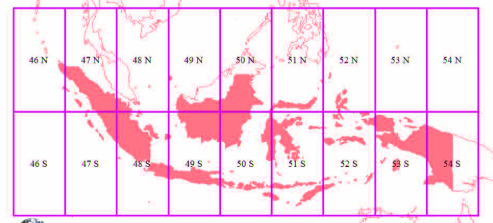
\includegraphics[width=4cm]{figures/1174095/dzihan.png}
	\centering
	\caption{Pembagian Zona Waktu}
\end{figure}

\subsection{Data Geospasial}
Data spasial adalah data yang memiliki referensi ruang kebumian (georeference) di mana berbagai data atribut terletak dalam berbagai unit spasial. data spasial  sangat penting untuk perencanaan pembangunan dan pengelolaan sumber daya alam.
Data spasial terbagi menjadi dua yaitu :
Data vektor adalah data yang direpresentasikan sebagai suatu mosaik berupa garis, polygon, titik/point, dan nodes. Salah satu keuntungan dari format data vektor adalah akurasi dalam merepresentasikan fitur titik, batasan dan garis lurus.

Data Vektor berguna untuk analisa yang membutuhkan ketepatan posisi, misalnya pada basis data batas-batas kadaster. Contoh penggunaan lainnya adalah untuk mendefinisikan hubungan spasial dari beberapa fitur. vektor memiliki kekurangan yaitu ketidakmampuannya dalam mengakomodasi perubahan gradual.
	Data Raster
Data raster adalah data hasil dari penginderaan secara jauh. Data Raster sering disebut juga dengan sel grid. Dalam data raster obyek geografis direpresentasikan sebagai struktur sel grid yang disebut dengan pixel (picture element). Resolusi data raster tergantung pada ukuran pixel-nya .resolusi pixel menggambarkan ukuran sebenarnya di permukaan bumi yang diwakili oleh setiap pixel pada citra
\subsection{Link}
\href{https://youtu.be/KLmO0eBCJAQ}{Lihat Videonya disini}
\subsection{Plagiarism}
\begin{figure}[H]
	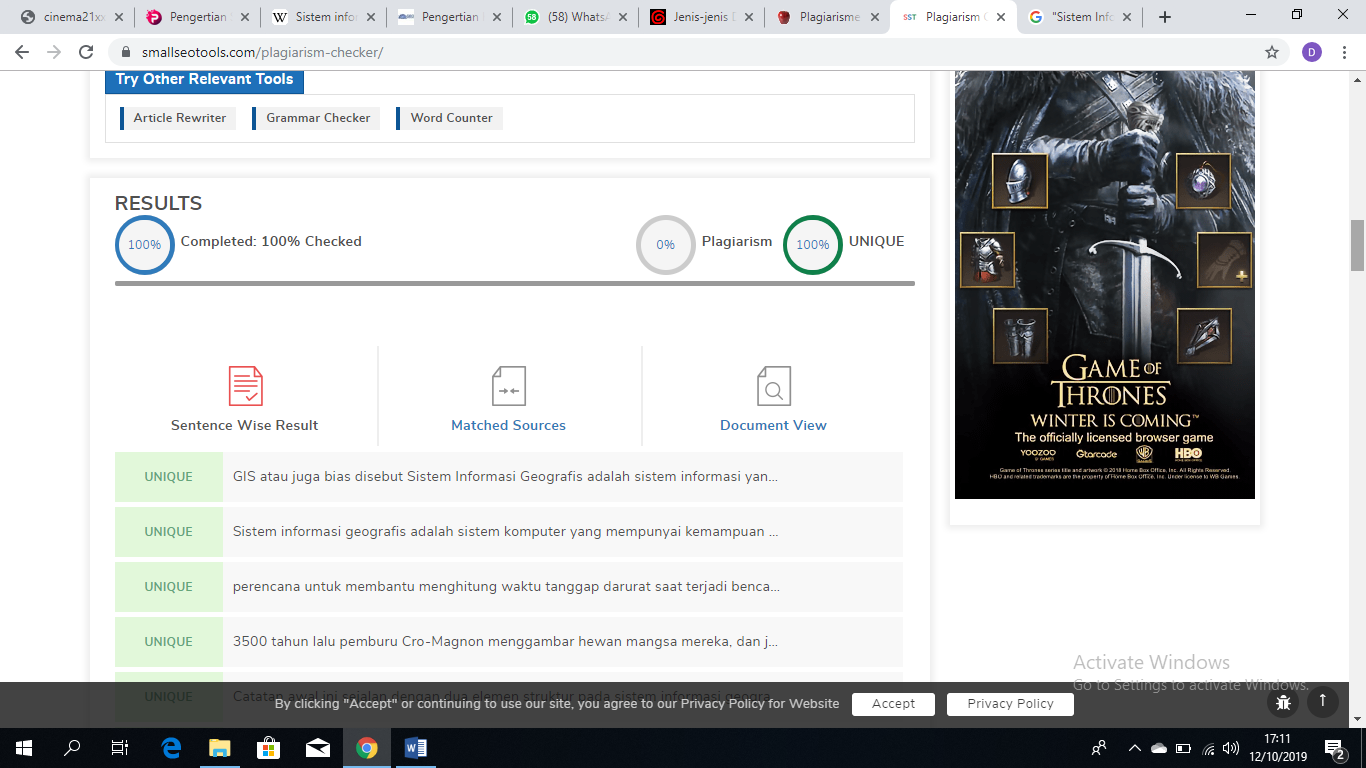
\includegraphics[width=4cm]{figures/1174095/plag.png}
	\centering
	\caption{Plagiarisme}
\end{figure}
